
\chapter{Theory of Correspondences}\label{chap3}

\setcounter{section}{6}
\section{Correspondences}\label{chap3:sec7}

\textbf{1.}~ In\pageoriginale this article we shall define so - called
correspondences of 
  Riemann surfaces, and study a class of special correspondences of
  the surfaces $s_{\mathcal{J}}$ to be defined below. They are certain
  operators and form a ring. In \S \ref{chap3:sec7} We shall study various
  representations of this ring. These representations are of
  topological, function theoretical or of arithmetical nature. We
  shall determine the traces of some of them  and this will load to
  several interesting arithmetical results.  

  Let $S$ and $S'$ be two closed Riemann surfaces and let $f$ be an
  analytic (algebraic) mapping.  in general multi-valued, of $S$ onto
  $S'$. If $P$ is a point of $S$, then $f(P)$ is a set of points of
  $S$, then $f(P)$ is a set of points $P'_1,  \ldots,  P'_d$,., of
  $S'$, said to this $f$ we associate the correspondence which we may
  write as  
  $$
  C : C(P) = P' _1 + \cdots + P'_d, ( \text{ formal sum }; 
  $$
  where it may happen that some $P' _i$ is equal to some $P' _j$. 
  
  If for $P' \in S' ,  f^{-1} (P')$ consists of $P_1,  P_2, \ldots,
  P_d$, then $f^{-1}$ gives rise to the correspondence  
  $$
  C^* : C^*(P') = P_1 + \cdots P_d. 
  $$
  

  We may view the correspondence as follows:

  Let $S''$ be the Riemann surface of the multi-valued function $f$,
  then $S''$ is compact and is covering surface of both $S$ and $S'$
  with $d'$ and $d$ sheets respectively. Let $\pi_1$ and $\pi_2$ 
 \begin{figure}[H]
    \centerline{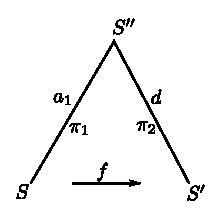
\includegraphics{vol9-figures/fig9-9.eps}}
  \end{figure}  
\noindent 
 be\pageoriginale  the corresponding projection maps. Then $f(P) =
  \pi _2 \pi^{-1}_1 
  (P)$ is the set of points $P'_1,  \ldots P'_d$, and similarly
  $f^{-1}(P') = \pi_1\pi^{-1}_2 (P')$. (It is easily seen that both
  $f$ and $f^{-1}$ are onto).  
 

As an example of a correspondence we consider the following figure:

  Here $d' = 2$, $d = 3$. 
  
  In the case that $S'$ is homomorphic to $S$, we show that we can
  make the set of correspondences of $S$ onto itself into a ring. So
  let $\nu$ be a homomorphism of $S'$ on $S$, i.e, $S'^\nu = S$. If
  $C$ is a correspondence between $S$ and $S'$ defined by $C(P)=P'_1, +
  \ldots + P'_{d'}$ then the correspondence $\nu C : S \to S $ is defined by  
  \begin{figure}[H]
    \centerline{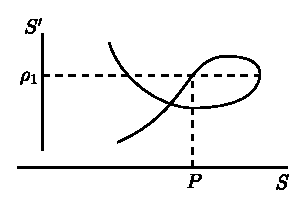
\includegraphics{vol9-figures/fig9-10.eps}}
  \end{figure}
  $$
  C(P) = (P'_1)^\nu + \cdots+ (P'_{d'})^\nu.  
  $$

  For such correspondence we can can define addition, ( in fact,
  addition, can be such defined for any two correspondences between $S$
  and $S'$ ) and multiplication in the following way: Let $D_1,  D_2$
  be two correspondences from $S \to S$. Then we define $(D_1 + D_2)
  (P) = D_1 (P)+(D_2) (P), (D_1 D_2) (P) = D_1 (D_2(P))$, and
  for any rational integer $n$, $(n D)$\break $(P) = n.  D (P)$ so that $(D_1 -
  D_2) = D_1 + (-1) D_2)$. There exists a zero correspondence, it maps
  each $P$ on the empty se, and the unit element is the identity
  map. Multiplication is associative and distributive with respect to
  addition,  so that the correspondence of $S$ on $S$ form a ring
  $\mathscr{R}$.  

  We\pageoriginale now prove the existence of an involution in
  $\mathscr{R}$. Consider the mapping $C \to C^*$   which is a $1-1$
  mapping of $\mathscr{R}$ onto $\mathscr{R}$. This mapping has the
  properties  
  \begin{enumerate}[1.]
  \item $(C_1 + C_2 )^* =C^*_1 + C^*_2 $
  \item $(C_1  C_2 )^* =C^*_2 C^*_1 $
  \item $C^{**} = C, $
  \end{enumerate}
  so that it is an involution in $\mathscr{R}$. 
  
  (This involutorial anti-automorphism is named after Rosati.)

\textbf{2.}~ We will now study the correspondence from
$S_{\mathcal{J}}\to S_{\mathcal{J}}$, where
  $\mathcal{J}$and $\mathcal{J'}$ are orders in $Q/k$.  ( For
  explanations and notations, see $\S 5$). To be precise,  let $Q$ be
  an indefinite quaternion algebra over the rational number field $k$,
  and $\mathcal{J}$ an order in $Q$. Let $Q_{\mathcal{J}}$ denote the
  proper unit group of $\mathscr{J}$, then $Q_{\mathcal{J}} = \left\{
  \begin{pmatrix}  \alpha & \beta \\ \gamma & \delta \end{pmatrix} =
  \varepsilon,  \quad  n (\varepsilon) = 1 \right\}$, where $\alpha,
  \ldots,  \delta $ lie in a real quadratic extension of $k$ which is
  isomorphic to a subfield of $Q$. Each element $\epsilon$ of
  $Q_{\mathcal{J}}$ gives 
  rise to  a linear transformations $z \to \varepsilon (z),
  \varepsilon \in Q_{\mathcal{J}}$.  

  \begin{remark*}
    Since $\pm \varepsilon \in Q_{\mathcal{J}}$ give rise to the same
    element of $\Gamma _{\mathcal{J}}, \Gamma _{\mathcal{J}}$ is not a
    faithful representation of $Q_{\mathcal{J}}$. It can be proved
    that $\Gamma_{\mathcal{J}}$ is a faithful representation
    $Q_{\mathcal{J}}/ _{ (\pm E)}$.  
  \end{remark*}
  
  The closed Riemann surface $S_\mathcal{J}$ associated with the group
  $Q_J$ can be considered as the compactifications of the quotient
  space of the upper half plane modulo $\Gamma _{\mathcal{J}} $, i.e.,
  $S_{\mathcal{J}}: \big\{ \Gamma_{\mathcal{J}}.  z,  z $ in the upper
  half plane
  $\big\}$. Similarly if $\mathcal{J}'$  is another order, we have the
  surface $S_{\mathcal{J}'}$,\pageoriginale and we will consider some special
  correspondences between $S_{\mathcal{J}}$ and $S_{\mathcal{J}}$. 

  Since $\mathscr{O}_{\mathcal{J}} \cap \mathscr{O}_{\mathcal{J}'}$ is
  of finite index in both $\mathscr{O}_{\mathcal{J}}$ and
  $\mathscr{O}_{\mathcal{J}'}$ (for a proof under similar 
  situation, see $P.46$). say $d'$ and $d$, the same holds for
  $\Gamma_\mathcal{J} $ and $\Gamma_\mathcal{J'} $.  Consequently we
  have the coset decompositions.  
  $$
  \Gamma_{\mathcal{J}} = \sum^{ d '}_{ i = 1} \Gamma_{\mathcal{J}}
  \cap \Gamma_{\mathcal{J'}}\epsilon_i = \sum^{d}_{ i = 1} (\Gamma_{\mathcal{J}}
  \cap \Gamma_{\mathcal{J}'} )\varepsilon'_i  
  $$

  Let $S_{\mathcal{J} \cap \mathcal{J'} }$ be the surface associated
  with $\mathscr{O} \cap \mathscr{O}_{\mathcal{J}}$, so that $S_{
    \mathcal{J} \cap \mathcal{J'}} : \{ \Gamma_{\mathcal{J}}\cap
  \Gamma _{\mathcal{J}'}z\}$, and $S_{\mathcal{J}}\cap \mathcal{J'}$,
  is a covering surface of both $S_{\mathcal{J}}$ and
  $S_{\mathcal{J}'}$ sheets $d'$ and $d$ respectively. Then the points
  lying over $\Gamma_{\mathcal{J}}.  z$ are precisely  
  $$
  \Gamma_{\mathcal{J}} \cap \Gamma_{\mathcal{J'}}. z_i,  z_i =
  \varepsilon _i (z), i = 1,  \ldots,  d'. 
  $$
  

  The correspondence $C_{S_{\mathcal{J}} \to S_{\mathcal{J}'}}$ is defined as 
  $$
  C_{S_{\mathcal{J}} \to S_{\mathcal{J}'}} (\Gamma_{\mathcal{J}.  Z})
  = \sum^{d'}_{ i = 1}\Gamma_{\mathcal{J}'} z_i 
  $$
  $C^* $ is given by 

  \hfill $C^\ast_{S_{\mathcal{J}'} \to S_{\mathcal{J}}}
  (\Gamma_{\mathcal{J}'}\cdot  z) = \sum^d_{i =
    1}\Gamma_{\mathcal{J}}\cdot \varepsilon'_i (z)$. 
  \begin{figure}[H]
    \centerline{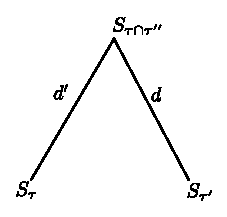
\includegraphics{vol9-figures/fig9-11.eps}}
  \end{figure}
\medskip

  We now restrict our attention to orders $\mathcal{J'}, \mathcal{J}$
  such that $\mathcal{J'}  \cong \mathcal{J}$ so that there exists
  $\nu \in Q$ such that $\mathcal{J} = \nu ^{-1} \Gamma_{\mathcal{J}}
  \nu $. Then $\Gamma_{\mathcal{J}'} = \nu^{-1} \Gamma_{\mathcal{J}}
  \nu$ and $C_{S_{\mathcal{J}}\to \mathcal{J}}, (\tau _{ \mathcal{J}.
  Z}) z = \sum^d_{ i = 1} v^{-1}\Gamma_{\mathcal{J}^ \nu}.Z_i $,  
  and 
  $$
  \nu C_{S_{\mathcal{J}}}\to S_{\mathcal{J}'} (\Gamma_{\mathcal{J}}.z)
  =\sum^{d'}_{ i = 1} \Gamma_{\mathcal{J}}\cdot \nu \epsilon_i z,  
  $$
  since $\Gamma _{\mathcal{J}}. \nu \epsilon_j =
  \Gamma_{\mathcal{J}}\cdot \nu \varepsilon _i,
  \varepsilon,  \varepsilon  \in \Gamma_{ \mathcal{J}}$ (for from a
  later lemma, it would follow that $\mathcal{J} \nu \varepsilon _i
  \varepsilon = \mathcal{J} \nu \varepsilon_j$) we can look upon $\nu
  C_{S_\mathcal{J} \to S_{\mathcal{J}'}}$\pageoriginale as a correspondence of
  $S_\mathcal{J}$ with itself, i.e.,
  $$
  C(\Gamma_{\mathcal{J}} \cdot z) = \sum\limits^{d'}_{i=1}
  \Gamma_{\mathcal{J}} \cdot \nu \varepsilon_i \cdot
  \Gamma_{\mathcal{J}} \cdot z,
  $$
  so that $C= \sum\limits_{i=1}^{d'} \Gamma_{\mathcal{J}}\cdot
 \nu \varepsilon _i$ may be
  considered as an operator on $S_{\mathcal{J}}$.  

  Therefore correspondences can be written as left operators 

\textbf{3.}~ Before defining modular correspondences, we shall prove an
  important lemma, which will enable us to pass from the topological
  aspect of correspondences to its algebraic counterpart. An element
  $\nu \in \mathcal{J}$ is said to be \textit{ primitive } if there
  exists no rational integer $t > 1$ such that $\dfrac{\nu}{t} \in
  \mathcal{J}$.  

\begin{lemma*}
  Let $\mathcal{J} $ be an order of the type $(q_1, q_2)$ and $n
  \chi| q_1, q_2$. If $\mathcal{J'} = \nu ^{-1} \mathcal{J} \nu$ and
  $\Gamma _{\mathcal{J}} = \sum\limits^d _{ i = 1} \Gamma _\mathcal{J} \cap
  \Gamma _\mathcal{J}. \varepsilon _i $, then all primitive
  (integral ) left ideals with norm $n$ are of the form $\mathcal{J}
  \nu \varepsilon _i (i = 1 ~\text{to}~ d ' )$ 
\end{lemma*}

\begin{proof}
  For such an order $\mathcal{J}$, the class number is $1$, so that
  every ideal is principal.  
\end{proof}

We shall not prove the lemma in its most general form but for
simplicity, assume that there are no characteristic primes, i.e., $q_1
= 1$. We may then take the order $\mathcal{J} =  \begin{pmatrix}
  \mathscr{O} & \mathscr{O} \\ q_2 \mathscr{O} &
  \mathscr{O}\end{pmatrix}$ ($q_2$ being square free).  

Let $\mu$ be a primitive left ideal for the order $\mathcal{J}$ with
norm $n$, so that in the reduced form, $\mu =
\mathcal{J}  \begin{pmatrix} n_1 & n_2 \\ 0 & n_3 \end{pmatrix}; n_1,
n_3 = n~  n_1 > 0 $  and $n_3 > 0, \quad n_2 $ is reduced modulo $n_3$,
$\mu$ being primitive $(n_1, n_2, n_3, ) = 1$.  

For our lemma, it is enough to show that there exists a unit
$\varepsilon$ such that\pageoriginale  
$$
\varepsilon~ \begin{pmatrix} n_1 & n_2 \\ 0 & n_3 \end{pmatrix}
= \begin{pmatrix} n & 0 \\ 0 & 1 \end{pmatrix} \varepsilon _ i ;
\text{For }\begin{pmatrix} n & 0 \\ 0 & 1 \end{pmatrix} 
$$
being a primitive element with norm $n, \varepsilon ' \nu
= \begin{pmatrix} n & 0 \\ 0 & 1 \end{pmatrix} {\epsilon _j }$
for some $\varepsilon'$ and $\varepsilon_j$, so that
$\mathcal{J} \begin{pmatrix} n_1  & n_2 \\ 0 & n_3 \end{pmatrix}
=\mathcal{J} \nu \varepsilon^{-1}_{ j}\cdot \varepsilon_i $. In fact,
we shall only prove that there exists units $\varepsilon,  \eta, \in
\Gamma_{\mathcal{J}}$ such that ${\varepsilon}{ \begin{pmatrix} n_1 &
    n_2 \\ 0 & n_3 \end{pmatrix}= \begin{pmatrix} n & 0 \\ 0 &
    1 \end{pmatrix}} \eta $ for, then writing $\eta = \eta _\circ
\varepsilon_i, \eta _\circ \in \Gamma_{\mathcal{J}}\cap \Gamma_{
  \mathcal{J}'},  \begin{pmatrix} n & 0 \\ 0 & 1 \end{pmatrix} \eta
_\circ = \varepsilon_\circ \begin{pmatrix} n & 0 \\ 0 &
  1 \end{pmatrix},  \epsilon \cdot \in \Gamma _\mathcal{J}$ 
we have 
$$
\varepsilon^{-1}_\circ  \varepsilon \quad { \begin{pmatrix} n_1 & n_2 \\ 0
    & n_3 \end{pmatrix} = \begin{pmatrix} n & 0 \\ 0 &
    1 \end{pmatrix}} \varepsilon_i.   
$$

Let $(n_2, n_3) = n_4$. Then $(n_1, n_4) = 1 $. Choosing $\gamma$ such
that $(\gamma,  n_3 ) = 1$, we see that $q_3 n_1 \gamma$ and $ n_4$
being coprime, we may find a unimodular matrix. $\begin{pmatrix} a & b
  \\ q_2 n_1 \gamma  & n_4 \end{pmatrix}$. With this matrix, we form
the product  
$$
\begin{pmatrix} n & 0 \\ 0 & 1 \end{pmatrix} \begin{pmatrix} a & b
  \\q_1 n_1 \gamma & n_4 \end{pmatrix} = \begin{pmatrix} n_1 n_3 a  &
  nb \\ q_2 n_1 \gamma  & n_4 \end{pmatrix}. 
$$
Again,  since $(a,  q_2,  n_1 \gamma) = 1$, i.e., $(a, q_2 \gamma) =
1$ and $(q_2 \gamma.,  n_3) = 1$, there exists a unimodular matrix
$\begin{pmatrix} A & B \\ -q_2 \gamma  & n_3   \end{pmatrix}$ so that  
$$
\begin{pmatrix} A & B \\ -q_2 \gamma  & n_3
  a  \end{pmatrix} \begin{pmatrix} n_1 n_3 a  & nb \\ q_2 n_1 \gamma
  & n_4 \end{pmatrix} = \begin{pmatrix} n_1  & Anb + Bn \\ 0 &
  n_3 \end{pmatrix} \sim \begin{pmatrix} n_1  &Bn_4 \\ 0 &
  n_3 \end{pmatrix} 
$$
where\pageoriginale ``$\sim $'' means that each matrix goes over into the other by
multiplication on the left by a unit of the type $\begin{pmatrix} 1 &
  t \\ 0 & 1 \end{pmatrix}, t$ begin a multiple of $n_3$. Further  
$$
\begin{pmatrix}
  n_1 & Bn_4 \\
  0 & n_3 
\end{pmatrix}
\sim 
\begin{pmatrix}
  n_1 & n_2\\
  0 & n_3
\end{pmatrix}
$$
for we may choose for $\gamma$, then element given by
$$
\gamma \frac{n_2}{n_4}. q_2 + \Lambda n_3 = 1
$$
$(q_2. \dfrac{n_2}{n_4}$ and $n_3$ are co-prime, since $(n, q_2) = 1$
implies $(n_3, q_2) = 1)$. Incidentally $(q_2 \gamma, n_3) = 1$ is
satisfied. Now, $B q_2 \gamma + An_3 a = 1$ implies that 
$$
B(1- \Lambda n_3) + An_3 a. \frac{n_2}{n_4} = \frac{n_2}{n_4}
\Rightarrow B n_4 \equiv n_2 \pmod{n_3} 
$$
which is what we required.

We have yet to show that any primitive ideal $\mathcal{J} \mu$ of norm
$n$ can occur only once among $\mathcal{J} \nu \varepsilon_i, i = 1$
to $d'$. For, if $\mathcal{J} \nu \varepsilon = \mathcal{J} \nu
\varepsilon'$, $\varepsilon, \varepsilon'$ two among $\varepsilon_1,
\ldots,  \varepsilon_d$, then it follows that $\nu \varepsilon =
\varepsilon'' \nu \varepsilon'$, i.e., $\varepsilon \varepsilon'^{-1} =
\nu^{-1} \varepsilon'' \nu \in \Gamma_{\mathcal{J}'}$ and also in
$\Gamma_{\mathcal{J}}$ so that $\varepsilon \varepsilon'^{-1} \in
\Gamma_{\mathcal{J}'} \cap \Gamma_{\mathcal{J}}$. The units that give
rise to the same ideal lie in the same coset modulo $\Gamma_{\mathcal{J}} \cap
\Gamma_{\mathcal{J}'}$, and conversely. Therefore there can be only
$d'$ distinct ideals of the type $\mathcal{J} \nu \varepsilon_i, i =
1$ to $d'$. 

Let $\nu$ be a primitive element of norm $n, (n, q_1 q_2) = 1$ of the
order $\mathcal{J}$. Let $\mathcal{J}' = \nu^{-1} \mathcal{J} \nu$,
then we have the correspondence of $S_\mathcal{J}$ onto itself defined
by 
$$
C_n = \sum^{d'}_{i = 1} \Gamma_\mathcal{J} \nu \varepsilon_i
$$
($\epsilon_i$\pageoriginale as defined in the above lemma). By the above lemma,
$$
C_n = \sum^{d'}_{i = 1} \Gamma_\mathcal{J} \cdot \nu_i
$$
where $\mathcal{J} \nu_i, i=1, \ldots,  d'$ are precisely all the
primitive integral ideals of norm $n$. (We may define $C_n$ even when
$(n, q_1 q_2) \neq 1)$. We call $C_n$ a\textit{ primitive modular
  correspondence. A modular correspondence} $T_n$, for $(n, q_1 q_2) =
1$, is defined by 
$$
T_n = \sum_{i} \Gamma_{\mathcal{J}} \cdot \mu_i
$$
where $\mathcal{J} \mu_i$ runs over all the integral left ideals with
norm $n$. (We know that this number is finite). We can now write 
$$
T_n = \sum_{t^2 / n} \frac{C_n}{t^2}
$$
for if $\mu \in \mathcal{J} $ is an element whose norm is $n$, then we
can write $\mu = \nu t, t \ge 1$, and $\nu$ is primitive $n (\nu) = n/
t^2$ and then  
$$
\Gamma_{\mathcal{J}} \mu = \Gamma_{\mathcal{J}}, \nu t = \Gamma_{\mathcal{J}}. \nu
$$
as an operator. Conversely if $\nu$ is a primitive element of norm
$\dfrac{n}{t^2}$ then $\mu = \nu.  t$ is an element of norm $n$, and
$\Gamma_\mathcal{J}. \nu t = \Gamma_\mathcal{J} \nu $ as an operator. 

\textbf{4.} ~\textit{Some properties of} $T_n$ : Let $T_n ^*$ denote the
inverse operator of $T_n$. Then 
\begin{enumerate}[1)]
\item $T_n ^* = T_n$
  (This will imply that the ring of operators $T_n$ is commutative).
\item $T_n.  T_m = T_{nm}$ if $(n, m) = 1$.
\item $T_{p^s}\cdot T_p t = \sum\limits^{\min (s, t)}_{\sigma = o}
  p^\sigma. T_p s + t - 2 \sigma$ 
\item $T_n.  T_m = \sum_{d | (n, m)} d. \dfrac{T_{nm}}{d^2}$
\end{enumerate}
for\pageoriginale any $n, m$. We shall prove these now.

1)~ We shall show first that $C^*_n = C_n$ and this will imply that
$T^*_n = T_n$, for since $T_n = \sum\limits_{t^2 | n} C_{n / t^2}$, we have 
$$
T^*_n = \sum_{t^2| n} C^*_{n/t^2} = \sum_{t^2| n} C_{\frac{n}{t^2}} = T_n.
$$

\noindent \textbf{Proof of} $C_n = C^*_n$.

Let $\tau, \sigma$ be two complex variables in the upper half plane.


By definition $C_n (\Gamma_\mathcal{J} \tau)  = \sum\limits_i
\Gamma_\mathcal{J} \nu_i \tau$. The elements in $C^*_n
(\Gamma_\mathcal{J}) \sigma$ contain those  $\Gamma_\mathcal{J}. \tau$
for which $C_n (\Gamma_{\mathcal{J}} \tau)$ contains
$\Gamma_\mathcal{J}. \sigma$, i.e., If $\Gamma_\mathcal{J} \tau \in
C^*_n\break (\Gamma_\mathcal{J} \sigma )$ then $\Gamma_\mathcal{J} \sigma =
\Gamma_\mathcal{J} \nu \tau$ for some $\nu \in \mathcal{J}$ of norm
$n$.  This means that $\varepsilon \sigma = \nu \tau $ or $\bar{\nu}
\varepsilon \sigma = n (\nu). \tau$ or $\Gamma_\mathcal{J}, \bar{\nu}
\varepsilon \sigma = \Gamma_\mathcal{J}. \tau$ as an operator in the
complex plane. By lemma in para $3$, as $\varepsilon$ runs over
$\Gamma_\mathcal{J}$, $\mathcal{J} \bar{\nu} \varepsilon$ runs over
all primitive left $\mathcal{J}$- ideals of norm $n$. Hence 
$$
C^*_n (\Gamma_{\mathcal{J}} \sigma) \nsupseteq \sum \Gamma_{\mathcal{J}}\cdot
\nu \sigma = C_n (\Gamma_\mathcal{J} \sigma) 
$$
and by symmetry, the other way, so that $C_n = C^*_n$. 

2) ~ $T_n.  T_m = T_{nm}$ if $(n, m) = 1$.

Let $T_n = \sum\limits_{i} \Gamma_\mathcal{J}. \nu_i, n (\mathcal{J}\,
\nu_i) = n$ and 
$$
\displaylines{\hfill
T_m = \sum^i_{k} \Gamma_{\mathcal{J}}\cdot \mu_k, \,n(\mathcal{J} \mu_k) =
m\hfill \cr
\text{hence} \hfill T_n. T_m = \sum\limits_{i, k} \Gamma_\mathcal{J} \nu_i
\Gamma_\mathcal{J} \mu_k = \sum\limits_{i, k} \Gamma_\mathcal{J} \nu_i
\mu_k.\qquad \hfill }
$$ 

Since the number of integral ideals of norm $n. m$ is $\sum\limits_{d
  | nm} d = \sum\limits_{d | n} d$.  $\sum\limits_{d' | m} d'$ (for ($n,
m) = 1$) (this follows from the factorization of ideals), and
conversely since any integral ideal $\mathcal{J} \nu_i \mu_k$ is of
norm $n. m$ if we prove that all these are distinct, our proof will be\pageoriginale
finished. So consider any two ideals $\mathcal{J} \nu_i \mu_k,
\mathcal{J} \nu_{i'} \mu_{k'}$, where $i \neq i'$ or $k \neq k'$. If $k
\neq k'$, let $p$ be a prime dividing $m$, then $(\mathcal{J} \nu_i
\mu_k)_p = \mathcal{J}_p \mu_k$, because $n(\nu_i) = n$ and $(n, m) =
1$, i.e., $n$ is a $p$-adic unit or $\nu_i$ is a unit in
$\mathcal{J}_p$. 

Similarly $(\mathcal{J} \nu_i, \mu_{k'})_p = \mathcal{J}_p
\mu_{k'}$. Now, since $k \neq k', \mathcal{J}_p \mu_k \neq
\mathcal{J}_p \mu_{k'} \Rightarrow \mathcal{J} \nu_i \mu_k \neq
\mathcal{J} \nu_{i'} \mu_{k'}$. If $k = {k'}, i \neq {i'}, \mathcal{J}_p
\nu_i \neq \mathcal{J}_p \nu_{i'}$, for at least one $p| n$ (for,
otherwise $\mathcal{J}_p \nu_i = \mathcal{J}_p \nu_{i'}$, for all $p,
\Rightarrow \mathcal{J} \nu_i = \mathcal{J} \nu_{i'})$, and then
$\mu_k = \mu_{k'}$ is a unit in $\mathcal{J}_p, \Rightarrow
\mathcal{J}_p \mu_i \mu_k \neq \mathcal{J}_p \nu_i, \mu_{k'}$; for
otherwise $\mathcal{J}_p \nu_i  = \mathcal{J}_p \nu_{i'}$. 

3) ~ $T_p s. T_p t = \sum\limits_{\sigma = o}^{\min (s, t)}
p^\sigma. T_p s + t - 2\sigma$ 

We will first prove that 
$$
T_p s. T_p = T_{p^{s+1}} + p. T_{p^{s-1}}
$$
and then obtain the required result by induction.

Let 
$$
\displaylines{\hfill 
  T_{p^s} = \sum_i \Gamma_\mathcal{J}. \nu_i, n (\mathcal{J} \nu_i) =
  p^s \hfill \cr 
  \text{and}\hfill 
  T_p = \sum_k \Gamma_\mathcal{J} \mu_k, n(\mathcal{J} \mu_k) = p;\hfill \cr
  \text{so that}\hfill 
  T_{p^s}. T_p = \sum_{i, k} \Gamma_\mathcal{J} \nu_i \mu_k =
  \sum_{\text{primitive}} + \sum_{\text{imprimitive}}.\hfill }  
$$

Because an integral ideal of prime power norm is uniquely decomposable
into prime factors if it is primitive, there occur, among the
$\mathcal{J} \nu_i \mu_k$ all integral primitive left ideals of norm
$p^{s + 1}$ exactly once. But,  if\pageoriginale $\mathcal{J} \nu_i \mu_k$ is
imprimitive it means that $\dfrac{\nu_i \mu_k}{\mathfrak{p}} \in
\mathcal{J}$, i.e., $\nu_i \mu_k = \nu'_i. p = \nu'_i \bar{\mu}_k
\mu_k \Rightarrow \nu_i = \nu'_i \bar{\mu}_k$. Since the number of
integral left ideals of norm $p$ is $p + 1$, there occur among
$\mathcal{J} \nu_i \mu_k$, all ideals $p \nu'_i \mathcal{J}$ of norm
$p ^{s + 1}, (p + 1)$ times each. Therefore, $T_{p^s}. T_p =
C_{p^{s+1}} + (p + 1) T_{p^{s-1}}$.  

Next, we have
$$
T_{p^{s+1}} = C_{p^{s+1}} + T_{p^{s-1}}.
$$

For,
\begin{gather*}
  T_{p^{s+1}} = \sum_{\text {prim. part }} + \sum_{\text {impr. part}}\\
  = C_{p^{s+1}} +  \sum \mathfrak{p} \Gamma_{\mathcal{J}} \eta
\end{gather*}
where the second sum is taken over all integral ideals $\eta$ with
norm $p^{s-1}$. The above sum therefore equals $C_{p^{s+1}} +
T_{p^s-1}$. 

From both the formulae, it follows that
\begin{center}
  \begin{fbox} 
    {$ T_{p^s} = T_{p^{s+1}} + p. T_{p^{s-1}}$} 
  \end{fbox}
\end{center}

We now use complete induction on $t$, i.e.,  assuming the result to be
true for $n \le t$, we prove it true for $t + 1$. (Without loss of
generality, we assume that $t \le s$). Now, 
$$
T_{p^s}. T_{p^t} = \sum_{\sigma = o}^{t} p^\sigma. T_{p^{s+t-2\sigma}}.
$$

Multiplying both sides by $T_p$, and substituting we have
$$
T_{p^s} (T_{p^t+1} + p. T_{p^{t-1}}) = \sum_{\sigma = o}^{t} p^\sigma
(T_{p^{s+t+1-2 \sigma }}+ p. T_{p^{s+1 - 1 - 2 \sigma}}) 
$$
\begin{align*}
  T_{p^{s}} T_{p^{t+1}} & = - p.T_{p^s}. T_{p^{t-1}} + \sum_{\sigma =
    o}^t p^\sigma T_{p^{s+t+1-2 \sigma}} + \sum_{\sigma = o}^t
  p^{\sigma + 1} T_{p^{s+t-1-2 \sigma}}\\ 
  & = - p \left\{ \sum_{\sigma = o}^{t-1}
  p^\sigma. T_{p^{s+t-1-2\sigma}}\right\} + '' \quad '' ~~ + ~ \cdots\\ 
  & = \sum_{\sigma = o}^t p^\sigma. T_{p^{s+t+1-2 \sigma}} +  p^{t+1} T_{p^{s-1-t}}\\
  & = 
  \begin{cases}
    \sum_{\sigma = o}^{t+1} p^\sigma.  T_{p^{s+t+1-2 \sigma}}, & \text { if } t < s. \\
    \sum_{\sigma = o}^t p^\sigma. T_{p^{s+t+1-2 \sigma}}, & \text { if } t = s,
  \end{cases}
\end{align*}
because\pageoriginale $T_{p^{-1}} = 0$ by convention.

Therefore, in either case,
$$
T_{p^s}. T_{p^{t+1}} = \sum_{\sigma = o}^{\min (s, t + 1)} p^\sigma. T_{p^{s+t+1-2 \sigma}}
$$
\begin{equation}
  T_n.  T_m = \sum{d | n, m} d.T_{n m / d^2} \tag{4}
\end{equation}

This follows as a direct consequence of the properties $(2)$ and
$(3)$. We may now define the operator $T_n$ for $(n, q_1 q_2) >
1$. Firstly, we shall define $T_p, p| q_1 q_2$ and then extend it to
$n$. 
\begin{enumerate} [1.]
\item $\underline{p | q_1}$. In this case, $\mathcal{J}_p$ is a
  maximal order in the division algebra $Q_p$, so that there exists
  only one integral ideal 
  $$
  \mathscr{P} \mathcal{J}_p \pi = \mathcal{J}_p \bar{\pi} = \bar{\pi}
  \mathcal{J}_{p} = \pi \mathcal{J}_{p} 
  $$
  with norm $p$ and hence the ideal $\mathcal{J} \pi = \bar{\pi}
  \mathcal{J} $ is the only integral ideal with norm $P$. 
  
  We define $T_p = \Gamma_{\mathcal{J}} \pi = \bar{\pi}
  \Gamma_\mathcal{J}$. Consequently $T_p. T_p = \Gamma_\mathcal{J} \pi
  \bar{\pi} \Gamma_\mathcal{J} = I$. Also $T_{p^s}. T_p =
  \Gamma_{\mathcal{J}} \pi^s.  \Gamma_{\mathcal{J}} \pi = ~
  \Gamma_{\mathcal{J}} \pi^{s+1} =  T_{p^{s+1}}$. 
\item $\underline{p \big | q_2}$. $\mathcal{J}_p \cong \begin{pmatrix}
  \mathscr{O}_p & \mathscr{O} \\ p \mathscr{O}_p &
  \mathscr{O}_p \end{pmatrix}$.  We\pageoriginale define $T_{p^n} =
  \sum\limits_{\nu} \Gamma_\mathcal{J} \nu$ where $\mathcal{J} \nu$
  are ambiguous ideals with norm $p^n$. But we have already shown that
  actually there is only one such ambiguous ideal. Now $\mathcal{J}
  \nu = \nu \mathcal{J}$, where $ \nu = \begin{pmatrix} 0 & 1 \\ p &
    0 \end{pmatrix}$. Hence $\mathcal{J} \nu^s = \nu^s \mathcal{J}$
  and $n (\nu^s) = p^s$. From this, we may deduce that there exists
  only one integral ambiguous ideal of norm $p^s$. 
\end{enumerate}

As before
$$
T_{p^s}. T_p = \Gamma_\mathcal{J}.  \nu^s.  \Gamma_\mathcal{J}.  \nu =
\Gamma_\mathcal{J}.  \nu^{s+1} = T_{p^{s+1}}. 
$$

Hence
$$
T_p. T_p = T_{p^2} = \Gamma_{\mathcal{J}} \cdot \nu^2 =
\Gamma_\mathcal{J} \begin{pmatrix} p & 0 \\ O & p \end{pmatrix} = I. 
$$

\noindent \textbf{Note}: We may deduce some interesting results from the above
multiplicative properties of $T_n$, regarding the representations of
the ring of operators $\mathscr{R}$ of $T_n$. 

\textbf{5.}~ Let $R(T_n)$ be the representation matrix of $T_n$ of some fixed
degree. Then, we have the following product formulae from $(2)$ and
$(3)$. 
\begin{enumerate}[1)]
\item If $ n, m$ are coprime to $q_1 q_2$ and $(n, m) = 1$, then
  $R(T_n T_m) = R(T_{nm})$. 
\item If $p \chi q_1 q_2, R(T_{p^s}.T_p) = R(T_{p^{s+1}})+ p. R(T_{p^{s-1}})$.
\end{enumerate}

For $p \big | q_1 q_2$, from the facts that $T_{p^2} = I$ and $
T_{p^s}. T_p = T_{p^{s+1}}$, we have $R(T_p. T_p) = R(T_{p^2}) = I$ and
$R(T_{p^s}. T_p) = R(T_{p^{s+1}}) $.
 
Consider now the $\zeta$-function associated with this
representation, as follows: 
$$
\zeta_R (s) = \sum_{n = 1}^\infty \frac{(R(T_n))}{n^s}.
$$

A\pageoriginale special representation is the one-rowed matrix $R(T_n) = R_1 (T_n)
=$ number of integral ideals with norm $n = \sum\limits_{d | n} d $
(if $(n, q_1 q_2) = 1)$. 

Hence
$$
\zeta'_{R_1} (s) = \sum_{(n, q_1 q_2) = 1} \frac{\sum_{d|n} d}{n^s} 
$$
(omitting in $\zeta_{R_1}$ those $n$ which are divisible by $q_2$).

This is easily seen to be the same as the $\zeta$- function,
associated with the order $\mathcal{J}$ but for those terms,
corresponding to the factors of $q_2$. We have seen that
$\zeta_{R_1}(s)$ possesses a functional equation. But it is still an
unsolved problem whether $\zeta_R (s)$ for an arbitrary $R$, possesses
a functional equation. 

We shall prove, using the multiplicative properties of $R(T_n)$ that
$\zeta (s)$ possesses an Euler product. It is easily seen that  
$$
\zeta_R(s) = \sum^{\infty}_{n = 1} \frac{R(T_n)}{n^s} = \prod_p (I +
\frac{R(T_p)}{p^s} + \frac{R(T_{p^2})}{p^{2 s}} + \cdots 
$$
\begin{enumerate}[i)]
\item In case $p \not\mid q_1 q_2$, we shall show that
  $$
  \sum^\infty_{n = o} \frac{R(T_{p^{n}})}{p^{n, \mathscr{S}}} = (I- R(T_p)
  p^{-s} + p^{1-2s})^{-1}. 
  $$ 
\end{enumerate}

For,  
\begin{align*}
   & \left(I + \frac{R(T_p)}{p^s} + \frac{R(T_{p^2})}{p^{2 s}} + \cdots
   \right)  (I - R (T_p). p^{-s} + p^{1-2s})\\ 
  & \qquad = \sum^\infty_{n = o} \frac{R(T_{p^n})}{p^{n s}} - \sum^\infty_{n =
    o} R(T_{p^{n+1}}).  p^{-(n+1)s}\\ 
  & \qquad - \sum^\infty_{n = o}
  R(T_{p^{n-1}}). p^{-(n+1) s+1} + \sum^\infty_{n = o} R(T_{p^n}). p^{-n
    s+1-2 s}\\ 
  & \qquad= I + \sum^\infty_{n = 1} R(T_{p^n}). p^{-ns} - \sum^\infty_{n = o}
  R(T_{p^{n+1}}). p^{- (n+1) s}\\ 
  & \qquad - \sum^\infty_{n = 1} R(T_{p^{n - 1}}). p^{- (n + 1) s+ 1}+
  \sum^\infty_{n = 1} R(T_p^{n -1}) p^{-n s + 1 - s}\\ 
  & \qquad = I.
\end{align*}

\noindent ii)\pageoriginale $\underline{p \big | q_1 q_2}$.
\begin{align*}
  \sum\limits^\infty_{n=0} R(T_{p^n}).  p^{- ns} & = I +
  R(T_p). p^{-s} + R(T_{p^2}). p^{- 2s} + \cdots\\  
  & = I + R(T_p). p^{-s} + p^{-2s} + R(T_p). p^{- 3 s} + \cdots\\
  & = (1+p^{-2s}+ p^{-4s} \cdots ) (I + R(T_p) p^{-s})\\
  & = \frac{I + R(T_p).  p^{-s}}{1 - p^{- 2s}}.
\end{align*}

Hence we have the Euler product
$$
\zeta_R (s) = \prod_{p \big | q_1 q_2} \frac{I + R(T_p). p^{-s}}{1 -
  p^{-2s}} \prod_{p+q_1 q_2} (I - R(T_p). p^{-s} +  p^{1-2s})
^{-1} 
$$

\section[Representations of the Modular...]{Representations of the Modular Correspondence by the Betti
  Groups}\label{chap3:sec8}%^sec 8 

\markright{8. Representations of the Modular Correspondence\ldots}

\textbf{6.}~ The chief task hereafter will be the determination of the traces
of certain representations $R(\mathfrak{M})$, $(\mathfrak{M}$, the
ring of correspondences or $T_n$ operators ) because the traces
determine the representations uniquely.  For some $R (\mathfrak{M})$,
the calculation of the trace leads to topological considerations, for
others traces are not yet known. For example, we shall be concerned
with the trace of the representation of $T_n$ by the Betti groups of
$S_\mathcal{J}$. 


  Let $S_{\mathcal{J}}$ be the Riemann surface associated with an order
  $\mathcal{J}$ and $S'_\mathcal{J}$ a homeomorph of
  $S_\mathcal{J}$. Let $C$ be a correspondence of $S_\mathcal{J}$, onto
  itself defined by means of the covering surface $S''$. It is easy to
  see from the definition of a correspondence, that $C$ takes cycles to
  cycles and boundaries to boundaries, so that $C$ induces an
  endomorphism of the Betti groups of dimension $0, 1$ and $2$. 
  \begin{figure}[H]
    \centerline{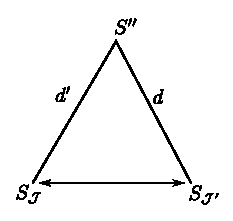
\includegraphics{vol9-figures/fig9-12.eps}}
  \end{figure}

Let\pageoriginale $T_n$ be a modular correspondence. Then $T_n = \sum\limits_{t^2/ n}
c_{\frac{n}{t^2}} C_{-s}$ being primitive correspondences and hence can be
looked upon as topological mappings of $S_\mathcal{J}$ onto
itself. Now, if we extend the notion of covering surface to include
disconnected pieces also, then $T_n$ may also be looked upon as a
correspondence in the topological sense. By  the above paragraph,
$T_n$ induces an endomorphism of the Betti groups $B^r (S), r = 0$, 1,
2 ; consequently, we have the traces of these endomorphisms, (say)
$tr^o (T_n), tr^1(T_n)$ and $tr^2(T_n)$. Here, $tr^1 (T_n) $= number
of sheets of $S''$ over $S =$ number of sheets of $S''$ over $S'$, both
being equal since $T_n = T^*_n$. Further 
$$
tr^o (T_n) = tr^2 (T_n) = \sum_{d | n} d ~\text{if } (n, q_1 q_2) = 1).
$$

For calculating $tr^1 (T_n)$, we apply Lefschetz's fixed-point theorem, namely

\begin{theorem*} % the 
~ %%

$\left.
  \begin{minipage}{4cm}
    The number $f(T_n)$ of fixed 
      points of $T_n$  with due  
      multiplicity
  \end{minipage}
  \right \}
  \begin{aligned}
    & = tr^o (T_n) - tr^1 (T_n) + tr^2 (T_n)\\
    & = 2 \sum_{d | n} d - tr^1 (T_n).
  \end{aligned}
  $
\end{theorem*}

We will calculate explicitly the left hand side so that we obtain
$tr^1(T_n)$ at once by the above equation. 

\textbf{7.}~ We\pageoriginale shall sketch a proof of Lefschetz's fixed - point theorem in
our case where $T_n$ are multi-valued analytic orientation preserving
mappings, by defining the multiplicities suitably, as the original
proof is rather lengthy and is not found in elementary text-books on
topology. 

We may define the multiplicity of a fixed point
$\Gamma_\mathcal{J}. \tau^o$, for a branch $\Gamma_\mathcal{J}
\nu_i$. This branch in the neighbourhood of this point can be expanded
as, 
\begin{align*}
  \tau_i = \nu_i (\tau) & = \nu_i (\tau^o) + c_1 (\tau -
  \tau^o)^{\frac{a}{b}} + c_2 (\tau - \tau^o)^{\frac{a+1}{b}}+
  \cdots\\ 
  & = \tau^o + c_1 (\tau - \tau^o)^{\frac{a}{b}} + c_2 (\tau -
  \tau^o)^{\frac{a+1}{b}}+ \cdots 
\end{align*}
(since $\nu_i (\tau^o)= \tau^o)$, where $\tau$ is a local uniformizing
parameter and $b$ being the common denominator of all the
exponents. Further $c_1 \neq 0$. The multiplicity of
$\Gamma_\mathcal{J} \tau^o$ as a fixed point is \textbf{${\min. (a,
    b)}$}.  

The general plan of the proof is to define a special linear mapping
$\varphi$ on the image of (a triangulation of ) $S_\mathcal{J}$, by
means of $T_n$, so that the mapping $\varphi(T_n)$ is homotopic to
$T_n$. Further $\varphi$ has to be boundary preserving. Since the
number of fixed points is invariant under homotopic deformations, it
is enough to calculate this number for $\varphi (T_n)$. 

We first cut up $S_\mathcal{J}$ into a finite number of triangles
$\tau^2_i$ (superscript meaning dimension), the fixed points being
among the vertices. We may choose the triangulation so fine that the
following conditions are satisfied: 

Let $\{\tau^j_i\} \,(j - 0, 1, 2)$ denote the simplices of the triangulation.
\begin{enumerate}[1)]
\item The\pageoriginale image $T_n (\tau^2_i)$ consist of a number of simply
  connected domains $\bar{\tau}^2_{ik}$ bounded by Jordan curves
  without double points. 
\item All images of each vertex are situated in the interior of some
  other triangle, except for the fixed points. 
\item All images of all points of a $\tau^2_i$ lie in such triangles
  $\tau^2_k$ which have no point in common with $\tau^2_i$, except for
  those $\tau^2_i$ which contain a fixed point. 
\end{enumerate}

Let $T_n (\tau^r_i) = \sum\limits_k \bar{\tau}^r_{ik}$ where
$\bar{\tau}^r_{ik}$ are, by $(1)$, simply connected domains $(r = 2)$,
arcs of curves $(r = 1)$ and points $(r = o)$. We shall now define a
linear mapping $\varphi $ on $\bar{\tau}^r_{ik}$ so that 
$$
\varphi_n (\tau^r_i) = \phi(T_n (\tau^r_i)) = \sum_k \varphi
(\bar{\tau}^r_{ik}) 
$$

The definition of $\varphi (\sigma^r) \,(r = 0, 1, 2)\,(\sigma^r$ are
cycles $\bar{\tau}^r_{ik})$ differs according as $\sigma^r$ contains a
fixed point or not. 

\noindent \textit {$i)$ Suppose first that $\sigma^r$ does not contain a fixed
  point.} 

Then
$$
\varphi (\sigma^2) = \frac{1}{3} \sum_j \varepsilon_j \tau^2_j
$$
where $\varepsilon_j$ is the number of vertices of $\tau^2_j$ lying in
$\sigma^2$. 
$$
\varphi(\sigma^1) = 
\begin{cases}
  \qquad  0  & \text { if } \mathcal{N} \text { lies entirely inside a
  } \tau^2_i.\\ 
  \frac{1}{6} \left(\tau'_1 + \tau'_2 + \cdots + \tau'_4\right) & \text { if }
  \sigma' ~\text{ crosses one boundary } 
\end{cases}
$$
once between two $\tau^2_i$, the sides being denoted as in the figure 

  Finally
  $$
  \varphi (\sigma^o) = \frac{1}{3} (\tau^o_{k, 1} +  \tau^o_{k, 2} + \tau^o_{k, 3}
  $$
  where $\tau^o_{k, j}$ are the vertices of a triangle
  $\tau^2_k$ in 
  which $\sigma^o$ lies.  
    \begin{figure}[H]
    \centerline{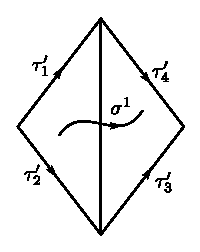
\includegraphics{vol9-figures/fig9-13.eps}}
  \end{figure}

By\pageoriginale linearity,
\begin{equation}
  \varphi (\sigma^r_1 + \sigma^r_2) = \varphi (\sigma^r_1) + \varphi
  (\sigma^r_2) \tag{*} 
\end{equation}
$\varphi$ is extended to all $\sigma^r$. $(r = 0, 1, 2)$.

We need not define $\varphi (\sigma^r)$ for $r = 0, 1$ when $\sigma^r$
has a point in common with a vertex $\tau^o_i$ because of the
assumptions made on.  $p. 99$ 
 
It is verified easily that the above definition of $\varphi $ on
$\sigma^r (r = 0, 1, 2)$ is consistent with linearity. It is also seen
that  
 $$
 \varphi (Bd (\sigma^r )) = Bd \,(\varphi (\sigma^r)).
 $$

  For example, when $r = 1$, $Bd \sigma^1 = A_2 - A_1$ and 
  \begin{align*}
    \varphi  (Bd \sigma^1) & = \varphi (A_2) - \varphi (A_1)\\
    & = \frac{1}{3} (B_2 + \not{B}_3 + \not{B}_4 - \not{B}_3 -
    \not{B}_4- B_1)\\
    & = \frac{1}{3} (B_2 - B_1).
  \end{align*} 
   \begin{figure}[H]
    \centerline{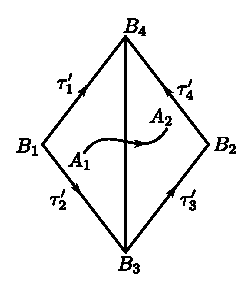
\includegraphics{vol9-figures/fig9-14.eps}}
  \end{figure}

  Now, $\varphi (\sigma') = \dfrac{1}{6} (\tau'_1 + \tau'_2 +
  \tau'_3 + \tau'_4)$ so that 
  \begin{align*}
    Bd \varphi (\sigma') & = \frac{1}{6} (\not{B}_4 - B_1 + \not{B}_3
    +B_1 + B_2 - \not{B}_3 + B_2 - \not{B}_4)\\ 
    &  = \frac{1}{3} (B_2 - B_1),
  \end{align*} 
 
i.e., $\underline(Bd (\varphi (\sigma^1 = \varphi (Bd (\sigma^1)$.
  
It is to be noted that the above definition of $\varphi$ is not to be
applied if $Bd \,\sigma^r$ passes through a vertex of a $\tau^2_i$,
which case we deal with later. 

Then, we have the following lemma (if $\sigma'$ does not pass through
a fixed point). 
  
\begin{lemma*} % lem 
  For\pageoriginale a closed curve $\sigma'$ without double points (in the usual
  sense), $\varphi (\sigma')$ is a cycle homotopic with $\sigma'$,
  (the triangulation being sufficiently fine). 
\end{lemma*}  

\begin{proof} % pro
  If the $\tau^2_i$ are sufficiently small, then the strip of
  simplices through which $\sigma'$ passes does not contain any
  double points. Then $\varphi (\sigma')$ can be obtained as follows:
  ($2$ arrows indicating traversed twice in the same direction). 
  \begin{multline*}
  \varphi (\sigma') = \frac{1}{3} \left[ (P_1 P_2) + (P_2 P_3) +
    \cdots + (P'_1 P'_2) + (P'_2 P'_3)\right. \\
    \left.+ \cdots + (P'_1 P_1) + (P_1
    P'_4) + (P'_4 P_2) \cdots \right] 
  \end{multline*}
   \begin{figure}[H]
    \centerline{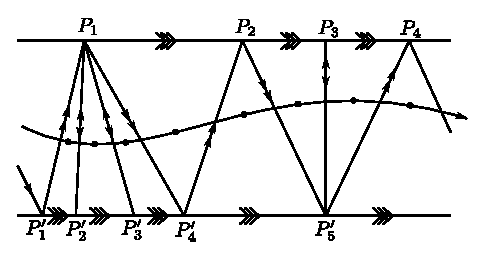
\includegraphics{vol9-figures/fig9-15.eps}}
  \end{figure}  
  and the lemma follows. $\sigma'$ passing through a fixed point will
  be taken up in case $(ii)$ after defining $\varphi$ in the
  neighbourhood of a fixed point. $(ii) ~ \sigma^r (r = 0, ~ 1, ~2)$
  \textit{contains a fixed point } $P$ (say). 
\end{proof}  
  
Because of linearity, it suffices to define $\varphi$ for such
$\sigma^\nu$ which are contained in the union of all $\tau^2_i$ having
$P$ as a vertex and this is called the star of $P$. 
  
We then define $\varphi (\sigma^2) = \dfrac{1}{6} \sum\limits_{j} \epsilon_j
\tau^2_j$ where $\varepsilon_j$ is the number of sides originating
from $P$ which pass through $\sigma^2$.\pageoriginale 
  
  Applying the linearity property $(*)$ we can assume without loss of
  generality that $\sigma'$ has no common points except $P$ with any
  $\tau'_{i, j} (j = 1, ~ 2)$ \,($\tau^2_i$ being the triangles through
  which $\sigma'$ passes) originating  from $P$. We then define 
   \begin{figure}[H]
    \centerline{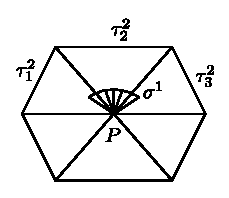
\includegraphics{vol9-figures/fig9-16.eps}}
  \end{figure}
  $$
  \varphi (\sigma') = \frac{1}{3} \left(\tau'_{i, 1} + \tau'_{i, 2}\right);
  $$
  $\tau'_{i, j}$ being the sides originating from $P$ of $\tau^2_i$
  through which $\sigma'$ passes. Finally $\varphi (P) = P$. 
     \begin{figure}[H]
    \centerline{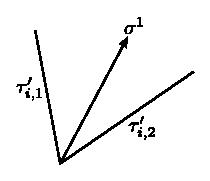
\includegraphics{vol9-figures/fig9-17.eps}}
  \end{figure}

  As before, consistency with linearity is verified and also the
  commutativity with the boundary mapping. Now, the above lemma is
  valid even if $\sigma'$ passes through a fixed point, with the
  above definition and is easily seen to be true. 
  
  We have then in either case $\varphi (T_n (\sigma^r)) \sim T_n
  (\sigma^r)\, (r = 0, 1, 2)$. For $r=0$ and $2$, this follows from the
  definition of $\varphi$ which is homotopic to the identity, and for
  $r = 1$, $\varphi (\sigma') \sim \sigma'$ from our lemma. 
  
  It can be seen that at this stage the condition that $\sigma'$
  should not have double points can be dropped for otherwise we can
  split it into pieces in each of which there is no double point, and
  the above relation holds good for the sum. 
  
  Since $Bd (T_n (\tau^r_i)) = T_n (Bd (\tau^r_i))$ and $Bd (\varphi
  (\sigma^r)) = \varphi (Bd (\sigma^r))$ we have $Bd (\varphi_n
  (\tau^r_i)) = \varphi_n (Bd (\tau^r_i))$. 
  
  This enables us to apply the Euler-Poincar'e-Hopf formula
  $$
  s^o (\varphi_n) - s^1 (\varphi_n) + s^2 (\varphi_n) = f(\varphi_n) = t
  \pi^o (\varphi_n) - t \pi^1 (\varphi_n) + t \pi^2 (\varphi_n) 
  $$
  ($\sigma^i$ denoting the traces of endomorphisms in the chain groups).

We\pageoriginale know $T_n \sim \varphi_n$ so that $f(T_n) =
f(\varphi_n)$. Therefore it is enough to compute for the linear
mappings $\varphi_n$, the number 
$$ 
f(\varphi_n) = s^o (\varphi_n) - s^1 (\varphi_n) + s^2 (\varphi_n).
$$

Because of the condition $(3)$ on the triangulation, it is enough to
consider the effect of $\varphi_n$ on the simplices $\tau^r_i$
belonging to the stars of fixed points. 

From the expansion, $\tau_i = \tau_o + c_1 (\tau -
\tau)^{\dfrac{a}{b}} + c_2 (\tau - \tau)^{\dfrac{a + 1}{b}} + \cdots,
c_1 \neq 0$, it is seen that star of $P$ is mapped ``$b$'' times on
Riemann surface of ``$a$'' sheets lying over the neighbourhood of
$P$, the ramification (of order a) being at $P$. In case $a = b$, and
$|c_1| = 1$, the mapping is approximately a rotation and the image of
the star of $P$ is of the same size as the star of $P$. If $a > b$ or
$a = b$ and $|c_1| < 1$, the image of the star of $P$ lies entirely
inside of the star of $P$. If $a < b$ or $a = b$ and $|c_1| > 1$, the
image of the star of $P$ lies entirely outside the star of $P$. We
shall treat the above cases one by one. 

\noindent
\textbf { i)} ~$a = b$ and $|c_1| = 1$.

  Let the image of $\tau'_i$ be the dotted line $\bar{\tau}'_i$. We
  may subdivide the star of $P$ so fine ($\bar{\tau}'_i$ need not be
  straight lines) that $\bar{\tau}'_1$ lies inside a sector both of
  whose sides differ from $\tau'_i$. By such a procedure, we have, by
  definition of traces 
   \begin{figure}[H]
    \centerline{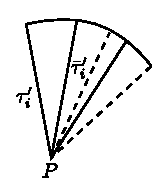
\includegraphics{vol9-figures/fig9-18.eps}}
  \end{figure}
$$
s^o (\varphi_n) = b, s^1 (\varphi_n) = 0, s^2 (\varphi_n) = 0
$$
regarding\pageoriginale the star of $P$. The first one follows from the fact that
$\varphi_n$ maps $P, ``b''$ times on itself. Hence the multiplicity of
the fixed point $P$ is given by  

$s^o (\varphi_n) - s^1 (\varphi_n) + s^2 (\varphi_n)$ (restricted to
the star $P$) 
$$
= b - 0 + 0 = b = \min  (a, b).
$$

\noindent
\textbf{ ii)}~ $a > b$ or $a = b$ and $|c_1| < 1$.

  In this case, the image of the star of $P$ lies completely inside the
  star of $P$ and we may deform $\varphi_n$ homotopically so as to make
  almost all images $\bar{\tau}^2_{ik}$ of $\tau^2_i$, sectors with an
  angle nearly zero at $P$ and the rest covering almost an angle $2
  \pi$. Further, we may take these to lie in $\tau^2_1$ (say) in a
  sufficiently small neighbourhood (see figure). 
   \begin{figure}[H]
    \centerline{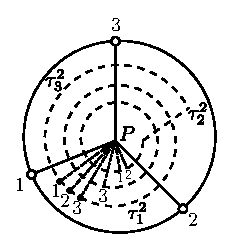
\includegraphics{vol9-figures/fig9-19.eps}}
  \end{figure}

(The broken lines show the $\bar{\tau}^r_{ik}$ ).
$$
(a = 3, b = 2),
$$

Only  $``a''$ of the $\bar{\tau}^2_{ik}$ (with $i \neq 1$) are sectors
of an angle nearly $2 \pi $. By our definition of $\varphi$, the
coefficient of $\tau^2_i$ in $\varphi_n (\bar{\tau}^2_{ik})$ is $0$ or
$\dfrac{1}{3}$ according as $\bar{\tau}^2_{ik}$ is a small or large
sector. 

Hence the contribution of the star of $P$ to $s^2 (\varphi_n)$ is
$\dfrac{a}{3}$. 

For\pageoriginale $s' (\varphi_n)$, by definition of $\varphi$ in the neighbourhood
of fixed point, the coefficient of $\tau'_{i, j}$ in $\varphi_n
(\tau'_{i, j})$ is $0$ or $\dfrac{1}{3}$ according as $i \neq 1$ or
$i = 1$. 

Furthermore, for each side $\tau^1_{i, 3}$ of $\tau^2_{i}$ opposite
to $P$ say $\tau^1_i, \varphi(\bar{\tau}^1_{ik}) = 0$ or
$\dfrac{1}{3}$ times the boundary of the star of $P$ according as
$\bar{\tau}^i_{ik}$ is small or large. Hence the contribution of the
star of $P$ to $s' (\varphi_n)$ is $(a + 2 b)/3$. 

Lastly $\varphi(P) = b. P$. and for other vertices $\tau^o_{i, k}$ of
the triangles $\tau^2_i, \varphi$ $(\bar{\tau}^o_{ik, j})=
\dfrac{1}{3}$ (sum of the vertices of $\tau^2_i$). Hence the
contribution to $s^o (\varphi_n)$ of these is $\dfrac{2b}{3}$, i.e.,
in the star of $P, s^o (\varphi_n) = b + \dfrac{2b}{3}$. 

Therefore
\begin{align*}
  s^0 (\varphi_n) - s^1 (\varphi_n) + s^2 (\varphi_n) & = \frac{a}{3} -
  \left(\frac{a}{3} + \frac{2b} {3}\right) + \left(b + \frac{2b}{3}\right)\\ 
  & = b = \min (a, b).
\end{align*}

\noindent
\textbf{(iii)}~ $a < b$ or $a = b$ and $|c_1| > 1$.

  Here the image lies completely outside the star of $P$. For
  simplicity, we consider only one large triangle. This is cut
  up into three parts as shown in the diagram. 
  For a large $\bar{\tau}^2_{ik}$, the coefficients of $\tau^2_i$ in
  $\varphi (\bar{\tau}^2_{ik})$ is $1$ and for small sectors, the
  coefficient is zero. So the contribution of the neighbourhood of $P$
  to $s^2 (\varphi_n)$ is a.  
   \begin{figure}[H]
    \centerline{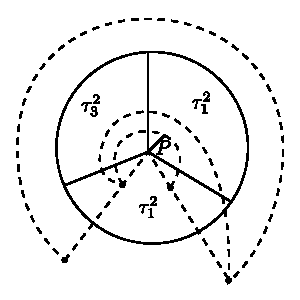
\includegraphics{vol9-figures/fig9-20.eps}}
  \end{figure}
\medskip

Now, the sides $\tau^1_{ik} (j = 1, 2)$ of $\tau^2_i$\pageoriginale originating in
$P$ are divided into two parts. The sides $\tau^{(1)}_{1, j}$ have
coefficients $\dfrac{1}{2}$ in $\varphi (\bar{\tau}^1_{ik, j})$, so
that the contribution from these is $b$ while other sides of $\tau^2_i$
have no contribution. 

Lastly, the only contribution to $s^o (\varphi_n)$ of the star of $P$
is given by $P$ and that is $b$. Hence we obtain  
$$
s^o (\varphi_n) - s^1 (\varphi_n) + s^2 (\varphi_n) = a - b + b = a =
\min (a, b). 
$$

For the full traces $s^o, s^1$ and $s^2$, summing up, for each fixed
point the multiplicity being $\min (a, b)$, we obtain finally the
result that  

\begin{equation*}
    \left.
  \begin{aligned}
    &\text{the number of fixed points}\\ 
    &\text{with due multiplicity}
  \end{aligned}\right\}
    = s^o (\varphi_n) - s^1 (\varphi_n) + s^2 (\varphi_n).
\end{equation*}
